\documentclass[12pt,pdftex]{article}
\usepackage{amsmath}
\usepackage{graphicx}
\usepackage{natbib}
\citestyle{elsart-harv}
\usepackage{rotating}
\usepackage{lineno} 
\usepackage{longtable}
\usepackage{amsmath}
\usepackage{amssymb}
\usepackage{subcaption}
\usepackage{setspace}
\usepackage{floatrow}
\floatsetup[table]{capposition=top}

% Text layout
\topmargin 0.0cm
\oddsidemargin 0.5cm
\evensidemargin 0.5cm
\textwidth 16cm 
\textheight 21cm

% Leave date blank
\date{}

\title{Conditions for successful range shifts under climate change -- the role of species dispersal and landscape configuration}
                                                                  
\author{Jonatan \r{A}revall$^{1}$,  Regan Early$^{2}$, Alba Estrada$^{3}$, \\ Uno Wennergren$^{1}$ \& Anna C Ekl\"{o}f$^{1*}$,\\
 $^1$\small Department of Physics, Chemistry and Biology, Division of Theoretical Biology,\\ \small  Link\"{o}ping University, Link\"{o}ping, Sweden, jonatan.arevall@liu.se\\
 $^2$\small Centre for Ecology and Conservation, University of Exeter Penryn Campus,\\ \small Cornwall, UK, R.Early@exeter.ac.uk\\
 $^3$\small Research Unit of Biodiversity (UMIB, UO-CSIC-PA), \\ \small Oviedo University – Campus Mieres, Spain, albaestradaa@gmail.com \\
% $^4$\small Department of Physics, Chemistry and Biology, Division of Theoretical Biology,\\ \small  Link\"{o}ping University, Link\"{o}ping, Sweden, uno.wennergren@liu.se\\
% $^5$\small Department of Physics, Chemistry and Biology, Division of Theoretical Biology,\\ \small  Link\"{o}ping University, Link\"{o}ping, Sweden, anna.eklof@liu.se\\
  $^*$ \small Corresponding author: anna.eklof@liu.se\\
}

\begin{document}
\linenumbers
\maketitle
\baselineskip 18pt
\begin{spacing}{2}

\subsubsection*{Corresponding author}
Anna Ekl\"{o}f\\
%Link\"{o}ping University\\ 
%Department of Physics, Chemistry \& Biology\\
%Link\"{o}ping, SWEDEN\\
email: anna.eklof@liu.se\\
phone: +46 (13) 282684\\
orcid.org/0000-0003-2721-0051\\


%\noindent {\bf Running title:} Conditions for successful range shifts\\ 
%
%\noindent {\bf Key words:} 
%climate change, dispersal, landscape configuration, point pattern, range shift, speed of climate change\\

\clearpage

\noindent{\bf Details}
\begin{itemize}
\item Article type: Biodiversity research
\item Running head: Conditions for successful range shifts
\item Abstract word count: 273
\item Main text word count: 4951 % No abstract, references, table or figure legends
\end{itemize}

\clearpage


\begin{abstract}
\noindent{\bf Aim:} Ongoing climate change is currently modifying the geographical location of areas that are climatically suitable for species. Understanding a species' ability to successfully shift its geographical range would allow us to assess extinction risks and predict future community compositions. We investigate how habitat configuration impedes or promotes climate-driven range shifts, given different speeds of climate change and dispersal abilities.

\noindent{\bf Location:} 
Theoretical, but illustrated with European examples.

\noindent{\bf Methods:}  We model how a species' ability to track a directional shift in climatic conditions is affected by: i) species' dispersal abilities; ii) speed of climatic shift; and iii) spatial arrangement of the habitat. Our modeling framework includes within- and between-patch population dynamics and uses ecologically realistic habitat distributions and dispersal scenarios (verified with data from a set of  European mammal species), and, as such, is an improvement of classical range shift models. 

\noindent{\bf Results:}  In landscapes with a homogeneous distribution of suitable habitats, all but the least dispersive species will be able to range shift. However, species with high dispersal ability will have lower population densities after range shift. In heterogeneous landscapes species' ability to range shift is far more variable and heavily dependent on the habitat configuration. This means that landscape configuration in combination with the speed of climate change and species dispersal abilities give rise to non-linear effects on population sizes and survival after a climatic shift.

\noindent{\bf Main conclusions:}  : Our analyses point out the importance of accounting for the interplay of species dispersal and the landscape configuration when estimating future climate impact on species. These results link ecologically important attributes of both species and their landscapes to outcomes of species range shift, and thereby long-term persistence of ecological communities.
\end{abstract}

\section*{Key words}
dispersal, landscape configuration, range shift, speed of climate change, habitat distribution

\clearpage

\section*{Introduction}
One of the most important factors determining how species are distributed around the globe is their tolerance of climatic conditions \citep{Thomas2010}. However, ongoing climate change is currently changing the locations of areas that are climatically suitable for species \citep{Loarie2009}, and there is clear evidence that these changes are indeed inducing shifts in the distributions for a wide variety of organisms \citep{Parmesan2003, Chen2011,Lenoir2015}. There are also several examples of species that have not been able to track changes in climatic conditions \citep{Maclean2011}, thereby facing the risk of eventually going extinct. Therefore species' capabilities of successfully tracking the changing climate have far-reaching consequences for biodiversity \citep{Thuiller2005a}. 

For most ecosystems around the world habitat loss, degradation and fragmentation are primary causes of species declines \citep{Fahrig2003, JoernFischer2006}. Climate change is predicted to increasingly interact with, and often intensify, the effects of these factors \citep{Doerr2011}. Ultimately, the survival of a population facing a changing climate depends on its ability to either adapt to the new conditions \citep{Hoffmann2011,Sentis2015} or successfully disperse and colonize new geographical areas \citep{Travis2013}.  Understanding how species distributions and persistence are likely to be affected by climate change, in combination with factors affecting dispersal and colonization success, is critical to inform effective conservation strategies in a changing world \citep{Gillson2013a}. 

Landscapes, natural as well as human-modified, can be viewed as geographical areas with suitable and unsuitable habitats for a given species combined in different densities and configurations. Since species dispersal is a process that connects discrete habitat patches together, the amount of habitat is naturally important for a successful colonization event, but so is the distribution of the habitat patches in the landscape \citep{Villard1999, Baguette2013}. In fragmented landscapes the amount of habitat and landscape connectivity are often linked to each other \citep{Villard2014} but the relationship is by no means a necessity \citep{Wang2014} as the same amount of habitat can be distributed in various ways and thereby give different degrees of structural connectivity in the landscape. When the landscape gets re-structured due to land-use modifications, e.g., becomes more fragmented, the negative effects of lower structural connectivity is especially pronounced for species with certain characteristics, such as strong adaptation to the historic landscape configuration (i.e., species whose habitats historically have been abundant and less fragmented) or low dispersal ability \citep{Martin2016}. Climate change may in turn cause both habitats and the matrix to decrease in quality \citep{Martin2016}, potentially leading to interaction effects between land-use and climate change \citep{Pielke2005}. Landscape configuration, the species dispersal ability, and quality of the new habitat jointly contribute to the realized connectivity (i.e. how structural connectivity is experienced by a given species) and ultimately determines the outcome of species dispersal \citep{Baguette2013, Borthagaray2014}. 

Species' ability to track a changing climate is also dependent on how fast the climatic shift is progressing \citep{Schloss2012a}, and there can be profound differences in the rate of change between biomes \citep{Stocker2013, Loarie2009}. Species that are able to disperse longer distances and at a faster pace should be better able to track a fast shift in climatic conditions compared to a species with slower and more limited dispersal \citep{Walther2002, Angert2011}, with implications for biodiversity and other features of community structure. Even though long distance dispersal often is rare, and survival and establishment commonly correlate negatively with the distance dispersed, long distance dispersal can have profound effects on species spread and survival \citep{Nathan2006} . 

Simulating biodiversity scenarios under climate change has so far largely relied on species distribution models, SDM, \citep{Guisan2000, Thomas2006a}, where statistical correlations between species' current distribution and a set of environmental variables are used to make predictions of future distributions. However, the accuracy of these models have been extensively debated \citep{Thuiller2013, Araujo2012a, Wiens2009} owing to limitations such as species dispersal often being considered unlimited or non-existent \citep{Peterson2001, Thuiller2005a} and the exclusion of population dynamics \citep{Zurell2009}. To address this limitations there has been a recent development of ``hybrid models'' which combine the classical SDM approach with, for example, simple dispersal or population dynamic models \citep{Ehrlen2015}. \cite{Zurell2016} recently tested the predictive performance of  models for range dynamics differing in their complexity, and found a clear advantage for models including dynamic approaches. There have also been several advanced software tools developed for simulating species migration rates \citep{Collingham1996} and range shifts \citep{Midgley2010, Schumaker2013}. These models are primarily developed for simulating dispersal of plant species, hence have successfully been used for that purpose \citep{Perez-Garcia2017}. 

We developed a theoretical modeling framework to address the implications of habitat configuration more broadly, and link the results to real life scenarios. Our framework allowed us the flexibility to choose the type of population dynamic model and to impose different types of habitat distribution. We used this framework to investigate the joint impact of species dispersal, habitat configuration in landscapes, and the speed of climatic shift on species' abilities to colonize and survive in new climatically suitable areas. We illustrate the implications of our results using the landscapes that four European mammal species' will encounter during climatically driven range shifts.



\section*{Methods}

We modeled how species' ability to track a directional shift in climatic conditions was jointly affected by: i) spatial arrangement of suitable habitats in the landscape; ii) characteristics of species' dispersal abilities (shape of dispersal kernel); and iii) speed of the climatic shift. We explored how these factors affect the patch occupancy and overall abundance of the range-shifting population.

\subsection*{Landscape generation}			
We first produced a set of artificial landscapes with clear differences in habitat aggregation. We generated landscapes using a method based on spectral density, following the methodology described in \cite{Lindstrom2011}, to produce neutral point pattern landscapes (NPPL). The NPPLs are primarily defined by three parameters: the number of patches ($n$), a continuity parameter ($\gamma$) and a contrast parameter ($\delta$). The continuity parameter determines the spatial autocorrelation over multiple scales, i.e., if areas with similar patch density are located close to or far from each other. The contrast parameter defines the size of the difference between areas with dense or sparse habitat distribution, i.e., is a measure of density dispersion. For a detailed description of the method see \cite{Lindstrom2011}. As we here focus on the aggregation of habitats in the landscapes we kept  $\delta$ constant and analyzed two values of $\gamma$. The combinations we used were [$\gamma$=0, $\delta$= 3] and [$\gamma$=2, $\delta$= 3], which produce landscape types that have their habitat organized in a clearly homogeneous (evenly distributed over the whole landscape) versus heterogeneous (clearly aggregated) manner. We hereafter refer to those combinations as homogeneous and heterogeneous landscapes respectively. Note that each habitat is a point and thus does not have a specific area, and therefore the aggregation stems from how close that patches (points) are in space. The number of habitat patches distributed in each landscape was 1000.

\subsection*{Population dynamics}
In each habitat patch the population dynamics were described by a modified Ricker equation \citep{Ricker1954}

\begin{equation}
N_{i}(t+1)= N_{i}(t)    e^{r_{i}(t)(1-\frac{N_{i}(t)}{K_{i}(t)})^c}	
\end{equation}	

where $N_{i,t}$ is the population density in patch $i$ at time $t$; $r_{i,t}$ is the intrinsic rate of increase in patch $i$ at time $t$; $K_{i,t}$ is the carrying capacity for patch $i$ at time $t$; and $c$ is a parameter that affects the population's responsiveness, i.e., whether the population shows over-compensatory or under-compensatory dynamics in response to $K$.  $K$  is set to 1000 individuals to ensure a low risk of extinction since we study mainly change in population density. The dynamics parameter $c$ is set to 0.1 such that the population has under-compensatory dynamics to avoid complicating dynamic behavior such as chaos and cycles as well as instability of the numerical methods. The intrinsic growth rate $r$ is defined by the number of births and deaths in a population. In order to incorporate demographic stochasticity into the model we let $r_{i,t}$ vary between time steps and different habitat patches. We modeled the stochasticity by modifying the number of births in patch $i$ at time $t$ using a Poisson probability function (expected value $r_{b}$ = 1.85),  while the number of deaths was held constant  ($r_{d}$ = 0.75) \citep{Melbourne2008}. We chose not to allow the $r$-value to vary further in order to limit parameter space, but our preliminary analyses showed limited effects of realistic variations in the $r$-value. 

\subsection*{Species dispersal}
After reproduction individuals moved between patches and this dispersal process was described with a distance dependent model similar to that of \cite{Lindstrom2009}. For each individual dispersing from patch $i$ a sample was made from a distribution of arrival probabilities. The probabilities of movement of individuals from patch $i$ to patch $j$ was defined by a dispersal kernel of which the probability mass was given by

\begin{equation}
	P_{ij}=  
	\begin{cases} 
		\frac{e^-(\frac{d_{ij}}{a})^b}{\sum_{j=1}^{n}e^{-(\frac{d_{ij}}{a})^b}}   
				& \quad \text{for } j = 1,2,...,n \text{ and } i\neq j  \\    
		0 & \quad \text{if } i=j
	\end{cases}
\end{equation}


where $d_{ij}$ is the distance between patch $i$ and $j$; $a$ and $b$ are parameters determining the shape and width of the dispersal kernel; and $n$ is the total number of patches. The dispersal kernel is normalized by dividing by the sum of all possible destinations \citep{Lindstrom2009}. The proportion of a population that disperses from patch $i$ to patch $j$ at time $t$ is given by $N_{i,t} \times \sigma$ where $\sigma$ defines the proportion of the total population dispersing. Here we set $\sigma$ to 0.5 (in order to reflect a behavior in a medium dispersive populations), and $b$ to 1 (in order to model the dispersal kernel as an exponential distribution) and $a$ is the parameter used to vary the width of the tail of species' dispersal kernels. A species dispersal kernel is a function that describes the probability of a species dispersing different distances \citep{Nathan2006}.

 We let $a$ take the values 0.002, 0.032, 0.064 and 2.048 -- hereafter referred to as dispersal group 1--4 respectively, where group 1 has the most thin-tailed dispersal kernel (i.e. no Long Distance Dispersal (LDD) events \citep{Nathan2006, Hovestadt2001}), and group 4 the most fat tailed kernel (many LDD events, for a visual description see Fig. 1).  The population density in patch $i$ at time $t+1$ with regard to dispersal between patches was therefore 

\begin{equation}
	N_{i}(t+1)=N_{i}(t)  (1- \sigma)  + \sum_{j=1}^{n}P_{ji}(N_{j}(t) \times \sigma) \qquad i\neq j
\end{equation}

% FIGURE 1  

\subsection*{Simulation of the climatic shift} 
To simulate a climatic shift we started by assuming that the species had its optimal climatic conditions at a certain point in the landscape. We also assumed that the species’ distribution was centered at that point. We assigned the maximum carrying capacity of the species to the climatically optimal position in the landscape and then let the carrying capacity decline with increased distance from that position. The decline was modeled as a normal distribution.  Note that in our model the carrying capacity is only determined by the climate. In order to incorporate some stochasticity environmental noise, $\varepsilon$, was added to the carrying capacities of the patches, modeled as white noise with mean 1 and standard deviation 0.05 following \cite{Logdberg2012}.

Two landscapes, with 500 patches each and the desired aggregation, were generated and then positioned adjacent each other. This means there were 1000 habitat patches in the whole landscape, and of these we let the 500 patches in the starting landscape be inhabited from start. The 500 starting patches were seeded with 100 individuals each and the populations were allowed to settle for the initial 100 time steps before we started to simulate the climatic shift. The climatic shift was simulated as a sliding window where the suitable climatic conditions move in a steady pace from south to north the landscape over time. The climatic shift was simulated at three different speeds: the complete shift took place over 20, 80 or 160 time steps which we here after refer to as fast, medium and slow speed respectively. The simulated speeds of climatic shift corresponds to 2.5, 0.625 and 0.3125 km/year respectively, assuming that each theoretical landscape  corresponds to a 50x50km grid-cell. These values are within the range observed in empirical data \citep{Loarie2009}.  Finally, after the climatic shift has stopped the populations were allowed to settle for 100 time steps before the simulation was halted.

The simulations were performed in MATLAB (R2014b, The MathWorks, Natick, MA, USA). For each combination of speed of climatic shift (fast, medium and slow), species dispersal abilities (dispersal group 1, 2, 3 and 4) and habitat aggregation (homogeneous, heterogeneous) 30 replicates were produced. Replicates varied in the distribution of habitat patches, the noise added to species growth rates $r$ and patch carrying capacities $K$. This resulted in 720 simulations in total. For a schematic description of the simulation flow see Fig. 2.

\subsection*{Analysis of population change}
We followed and recorded the changes in population densities in all habitat patches before, during, and after the climatic shift. The results were presented as the average density of the global population at the end of the simulation taken over the 30 landscape replicates. We additionally calculated the habitat occupancy (the fraction of habitat patches with surviving populations) before, during and at the end of each climatic shift. Note that the number of habitat patches occupied at the beginning of simulation was 500, and this refers to whole initial global population, i.e. when 500 patches are occupied the fraction of the habitats occupied is $1$. This means that the fraction could become larger than 1 as novel parts of the landscape could be colonized at a faster pace compared to the pace with which initial habitats were emptied. 

\subsection*{Differentiation of heterogeneous landscapes}
In the heterogeneous landscapes the habitats were aggregated according to $gamma$=2 (see section Landscape generation). As a result of the aggregation a technical issue arose: when habitats are aggregated large areas in the landscape have no (or very few) habitats. This leads to high variation in population density, depending on where the center of habitat aggregation is placed relative to the climate optimum. An aggregation close to the climate optimum will result in a higher net carrying capacity for the landscape, which in turn will give a higher net population in the landscape. To analyze the effects of these differences in placement of the aggregates on species survival and density, we divided the heterogeneous landscapes into three classes based on the fraction of habitat positioned in middle third of the landscape:  landscape of type A - 0--23\%, type B - 24--43\%  and type C- 44--100\% of total habitat positioned in the middle of the landscape (for example landscapes, see Fig. 6). We analyzed how the population density changes during and after the climatic shift in these different landscape configurations. 

\subsection*{Which parameters control the speed of range shifts?} 
In order to further disentangle the role of the different variables (dispersal kernel width, speed of climatic shift and landscape configuration) we used a regression tree approach, which recursively partitions the predictor variables to explain the variation in the response variable. Regression trees assess whether a response variable is associated with variation in a number of explanatory variables, can represent more complex interactions than multiple regression or ANOVA, and are robust to nonlinear relationships \citep{Death2000, Brose2005a}. As the response variable we used the fraction of the population remaining at the end of the simulations divided by the population size when it had settled right before the climatic shift started, i.e. after the initial 100 time steps. We chose this response variable as the populations settled at varying densities depending on their dispersal ability and the landscape configuration. In the regression tree we used four classes of landscapes: homogeneous and the three classes of heterogeneous landscapes (see above). For these analyses we use the {\em rpart} package in \textsf{R} (Version 3.2.2; R Core Team 2015). 



\section*{Results}
All three factors - habitat configuration, width of the species’ dispersal kernel and speed of climatic shift - had a clear effect on the survival success of local populations following a changing climate. In landscapes with a homogeneous distribution of habitat patches there was an abrupt shift at an intermediate level of dispersal; above this threshold a high proportion of the local populations survive, and below it the entire population goes extinct (Fig. 3). The same trend was also present in more heterogeneous landscapes although the transition was smoother with more intermediate levels of survival (Fig.4). In both cases the shift became less abrupt when the speed of climatic shifts was slower (from left to right in Fig. 3 \& 4). The number of local populations persisting (number of occupied habitat patches) was on average highest when species had intermediate or more fat-tailed dispersal kernels, but the densities of the surviving populations decreased when the dispersal kernel changed from intermediate to fat-tailed (Fig. 3 \& 4). 


Looking at how the densities of the surviving populations changed over time as the climatic shift progressed, we saw that there was a large difference in the variability of densities in homogeneous (Fig. 5) but especially in heterogeneous landscapes (Fig. 6). In heterogeneous landscapes species can have both higher or lower densities compared to those in homogeneous landscapes. When the climatic shift progressed faster, population densities decreased at a faster pace (red areas in Fig. 5 \& 6). After the shift was completed, species with a sufficiently high dispersal ability were able to reverse the earlier density decline and recover, whereas species with the lowest dispersal ability went extinct. Even when species did survive, they were not certain to recover to the same levels as before the shift, as seen in particular for species of dispersal group 4 (species with the most fat-tailed dispersal kernel analyzed here).


We classified heterogeneous landscapes into three types: A, B and C, in which an increasing proportion of habitat lies in the middle of the landscape to be crossed, see Methods). The landscapes of type A and B show the highest variation in global population density after the populations had settled but before the climatic shift started Fig. S3). Those landscape types also showed high variation after the climatic shift and final settlement. The most striking difference between the types of heterogeneous landscapes is that type A showed a clear trend of decreasing densities during the shift and also a clear recovery, while types B and C did not. Note that in some cases there was an increase in global population density after the climatic shift.     


The regression tree analysis confirmed that the species dispersal ability was the factor having the largest effect on the fraction of the both population persisting after the climatic shift (Table 1) and the global population density (Table 2). After dispersal ability the actual distribution of the habitat played a major role for the fraction of habitat patches occupied. 


\section*{Discussion}

Our analyses highlight interacting effects of landscape configuration, dispersal kernel shape, and speed of climate change on the persistence of populations during and after a climatic shift. The idea that the ability of species to reach new  climatically suitable areas will be hampered by fragmentation and habitat loss has been widely studied \citep{Thomas2004}. While previous focus has mainly been on the amount of habitat, we here show that the realized distribution of suitable habitat is crucial. This affects conservation planning decisions, e.g. which areas to protect or restore, in particular since climate change induce both decreased habitat availability and quality \citep{Martin2016}.


The difference in landscape configurations ranging from homogeneous to heterogeneous habitat distribution is also a range from low to high levels of habitat aggregation. Our analyses show that in landscapes where habitats are heterogeneously distributed, landscapes with the same level of aggregation show highly variable trends. A high level of habitat aggregation means that large, contiguous parts of the landscape contain no suitable habitat. The densities and persistence of the local populations are therefore dependent on the actual location of the habitat aggregates. If aggregates are situated far away from where the species has its optimal carrying capacity the persistence will be low. This because the habitat in the aggregate will have low climatic suitability, and thus low carrying capacity. On the other hand, if the aggregates are located in areas with climates close to the species climatic optimum, then population densities, and hence persistence, will be high. Note, however, that there can be situations where few habitats are found close to the species climatic optimum. In these cases, as climate change proceeds, the optimum moves its position and can, during the shift, reach areas where the habitat density is high. Thus, the climatic shift can in some cases have a positive effect on population density. Alternatively, the new position of the optimal climate could be situated in an area where little habitat is available. This further strengthens the argument that the distribution of habitats is more important than the amount of habitat alone, and that a continuous and well-connected distribution of suitable habitat throughout the landscape is a lower risk option for conservation strategies providing higher predictability. 


Our results also show that species with the second lowest dispersal ability indeed benefit from a habitat distribution where the amount of suitable habitat patches is high in the middle of the landscape, i.e. the part the species disperses over before reaching the new climatic suitable areas. Earlier studies on how protected areas for biodiversity conservation should be placed in the landscape, have shown the importance of well-connected dispersal pathways (dispersal chains) for species persistence  \citep{Phillips2008}, and how this is particular important for species with limited dispersal ability \citep{Williams2005}. 

However, species dispersal often has a cost: a dispersing individual or propagule might not find suitable habitat \citep{Bonte2012}. Therefore, while fat-tailed dispersal kernels can ensure a greater survival rate for a metapopulation as a whole by increasing the chance of reaching new patches, they can also result in lower population densities. Here we show that for species with fat-tailed dispersal kernels (LDD more common) the population is capable of moving with the range shift, but may still not reach the same densities after the climatic shift has stopped. This is due to the fact that much of the population moves to areas further away from the climatic optimum, and thereby the global species population will have lower density than a species with a more thin-tailed dispersal kernel. An intermediate dispersal ability has been found to maximize the survival of a specialist, long-lived plant under climate change \citep{Perez-Garcia2017}. Our work supports the existence of such a 'mid-distance optimum' for population parameters that reflect a range of life-histories. Having a fat-tailed dispersal kernel therefore does not necessarily optimize survival for species experiencing climate change in homogeneous or in highly aggregated landscapes. Instead, the optimal dispersal kernel is tightly coupled to the spatial distribution of habitat available for the species to occupy in areas with good climatic conditions. 


Some species are dependent on larger consecutive areas of suitable habitat in order to have viable populations, e.g. species that need large home ranges or have limited dispersal abilities \citep{Lindenmayer2013, Hanski2011}. Although this is not explicitly modeled here, areas with different geographical extents will possess different viabilities due to the similar carrying capacities, and reproduction rates, in adjacent habitat patches. One could assume that larger aggregates of habitat would jointly have a higher quality by functioning as single larger habitat patches. However, for this to be beneficial for species, the habitat aggregations must be located in areas with good climatic conditions. This is a situation in which a Single Large habitat aggregation could be inferior to Several Small habitat patches (reawakening the SLOSS debate).  Dividing conservation protection between a large number of smaller habitat patches increases extinction rates within patches, and requires accurate estimates of local extinction rates \citep{McCarthy2011, Donaldson2017}. However, in the context of climate change, a large number of smaller habitat patches maximizes the ability of species with a broad range of dispersal capacities to undergo range-shifts. 

 
The speed of climate change is highly uncertain \citep{Stocker2013} and will differ between biomes \citep{Loarie2009}. Interestingly, the speed of climate change had limited effect on the survival of local populations and both the landscape configuration and species dispersal ability were usually more important. Our results show it is feasible for all but the species with the lowest dispersal abilities to cross homogeneous landscapes, even under the fastest speed of climate change that we simulated. However, for species with restricted dispersal ability, the speed of climatic shift will have a large effect on persistence. This means that species that are sensitive to isolation effects, for example forest species reluctant to cross non-forest habitat, will be particularly prone to extinction in areas of rapid climate change \citep{Melles2011}. This trend has also been observed in marine systems. For example in ocean of southeast Australia, species with high dispersal capacity and ecological generalism have expanded their range \citep{Sunday2015}, whereas other species faced a higher risk of being stuck in unsuitable areas as climate changes.


Of importance for conservationists and other stakeholders is to be able to identify circumstances under which a species is likely to be particularly vulnerable to extinction (or become an invasive).  Fig. 7 summarizes the combinations of dispersal abilities for species and landscape configurations and highlights those that are of particular conservation concern. It is evident that species' dispersal patterns play a major role in range shifts, but also that combinations of landscape and dispersal ability can result in unintuitive outcomes. For example, under the medium speed of climatic shift, landscape type heterogeneous C (most of the suitable habitats are located in the middle third of the landscape) and species from dispersal group 2 (the second most narrow dispersal kernel), results in a much lower global population density than under higher or lower speeds. But also, if the habitat distribution is different, say the landscape is of type A instead, the same dispersal type species will have a different population level response. One can also see that for some combinations the final population size is much larger after the climatic shift (large dots in Fig. 7), with possible implications for the species to become a problematic invasive \citep[for a summary of potential mechanisms, see ][]{Hellmann2008}. One example of this is that a species in dispersal group 3 increases its population after a high speed climatic shift if a large amount of habitat is positioned where the new climatic optimum is, but will have a severely decreased population if habitat is more limited.    


In order to evaluate the relevance of our theoretical modeling approach to conservation we compared our results to empirical data from four European mammals; siberian flying squirrel {\em Pteromys volans}, chamois {\em Rupicapra rupicapra}, European hare {\em Lepus europeaus}, and brown bear {\em Ursos arctos}.  The species dispersal kernels were calculated from natal dispersal distances \citep{Whitmee2013}, and are within the range of those used in the theoretical analyses  (Fig. 1, see SI Appendix 1 for details).  We allowed each 50x50km grid-cell in the European study area to correspond to a theoretical landscape as defined in the Methods (for details see SI Appendix 1). In each 50km grid-cell, the 1km grid-cells in which vegetation is suitable for the study species are considered to be habitat patches. 50km grid-cells adjacent to the current range, that become climatically suitable from 1961-1990 to 2071-2100 were taken from calculations in (Morrison, L., et al. , (accepted), "Species traits suggest European mammals facing the greatest climate change are also least able to colonise new locations", Diversity and Distributions), using the Representative Concentration Pathway 4.5 and CNRM-CM5 global climate model.  We calculated the Clark-Evans habitat aggregation indices \citep{Clark1954} in each 50km grid-cell that could be colonized, and compared these to Clark-Evans indices in the theoretical landscapes. The indices for empirical landscapes ranged between 0.31 - 1.50 (average value 0.84), and indices for theoretical landscapes ranged between 0.56 - 1.18 (average 0.83) (SI Appendix 1, Fig. S2). The simulated speeds of climatic shift of 20, 80 or 160 time steps correspond to 2.5, 0.625 and 0.3125 km/year respectively.  These values indicate that the parameters used in our theoretical study are representative of real-world range-shift scenarios, and that the approach could be used to address specific conservation questions. Theoretical landscapes that have Clark-Evans indices that match the empirical landscapes have diverse population densities, and the color of the empirical landscapes is shaded light or dark depending corresponding to the areas in the inset graphs (Fig. 8). When the Clark-Evans index of landscape aggregation is below 0.9, the arrangement of habitat patches can result in drastically different population densities.  For the mammals studied, approximately half of the 50km grid-cells they could soon colonise have habitat aggregations that could result in either very high, intermediate, or zero population densities, depending on the specific habitat distribution. The European hare (dispersal group 2) has the potential to have the highest population densities in colonised grid-cells, whereas most habitat configurations would result in relatively much lower population densities for the Brown bear (dispersal group 4). 

A complicating aspect for conservation actions is that species are not sole actors in ecological communities but rather depend on other species for survival (e.g., prey species, mutualistic interactions). The synchrony in movements of interacting species during a climatic shift will determine future biodiversity scenarios - a species highly able to disperse and colonize under shifting climate may not be able to do so if, for example, their prey species has more limited dispersal and colonization capabilities ('biotic mismatch')  \citep{Chivers2017}. In more homogeneous landscapes this variation in density will likely be less pronounced. In this situation, as patches of relatively good quality can easily be reached even by species with lower levels of dispersal ability, and therefore biotic interactions are more likely to be kept intact. Our analyses further emphasize that predicting biotic mismatch will depend not only on species' dispersal abilities, but also on landscape configuration, since species with different habitat requirements experience landscape connectivity differently  \citep{Taylor1993}. Also, if climate change progresses rapidly, dispersal-limited species might be trapped in habitats with low climatic suitability, with negative repercussions for any species that depends on them for their ecological interactions.

We have showed that the actual distribution of habitat patches, not only the distances between them, is crucial for species to survive during climate change. This is borne out by the fact that even for the species that move furthest and fastest, the landscape structure can block movement completely. Within the range of parameters we investigated, which reflect the range of landscape characteristics and dispersal abilities of European mammals, all but the poorest dispersers can successfully cross landscapes where habitats are relatively evenly distributed. The future is less certain for all species in heterogeneous landscapes where suitable habitats are unevenly distributed. 


Our results pinpoint the importance of taking into account factors like fragmentation, land-use, and dispersal barriers across large geographical scales when performing biodiversity predictions and developing conservation strategies in the light of climate change. While the speed and amplitude of climate change is something we cannot change in the short-term, the configuration of the landscape in many cases is. Restoration of destroyed habitats as well as thoughtful organization of green infrastructure elements  \citep{Benedict2006} may be a possible solution for lowering the risks in the short-term.


\section*{Acknowledgments}
This research was funded by the ERA-Net BiodivERsA, part of the 2011 BiodivERsA call for research proposals. RE and A.Es acknokledge the ERA-Net
BiodivERsA, with the national funder FCT, through the project BIODIVERSA/00003/2011. A.Ek. acknowledge funding from Swedish Research Council grant number 2016-04919. A.Es. has a postdoctoral contract funded by the project CN-17-022 (Principado de Asturias, Spain). Catarina Meireles compiled data on dispersal kernels and habitat tolerances for European mammals. We thank Alyssa Cirtwill and Gy\"{o}rgy Barabas for useful comments on the manuscript. 

\bibliographystyle{ecography}
%\bibliography{../../../../bibtexFiles/RangeShiftMS}
\bibliography{RangeShiftMS}
\clearpage

\section*{Supporting Information}
SI-ConditionsSuccessfulRangeShifts.pdf

\section*{Author contribution}
AEk and UW originally formulated the ideas presented in this article. J\r{A} coded the theoretical model and preformed the simulations. J\r{A} and AEk preformed the analyses of the simulated data. RE and AEs obtained the empirical species data and preformed the  analyses of them. J\r{A} and AEk wrote the first draft of the manuscript and all authors contributed extensively to the preparation of the final version.

\section*{Biosketch}
Jonatan \r{A}revall is a PhD student at Link\"{o}ping University, particularly interested in examining interactions between population dynamics, landscape characteristics and species’ dispersal behavior, and how these together can affect population distributions. He is also interested in applying these results to increase the efficiency of green infrastructure projects in order to accommodate biodiversity in the future.

\clearpage

\section*{Figure legends}

{\bf Figure 1.} Shows dispersal kernels used in the model (colored lines) and the dispersal kernels for four European mammal species (dotted lines). The mammals are from bottom to top {\em Pteromys volans}, {\em Rupicapra rupicapra} and {\em Lepus europaeus} (lines are overlapping), and finally {\em Ursus arctos}. The x-axis show distances as landscape units (50km). \\

\noindent{\bf Figure 2.} Schematic description of the range shift simulation. In this example a landscape with totally 1000 habitat patches heterogeneously distributed is produced (1). The landscape is a combination of two landscapes consisting of 500 patches each;  each black dot in the figure corresponds to one habitat patch. Then the one half of the landscape (here the lower part, which in a species range shift scenario would corresponds to the south part) is populated with 100 individuals in each patch (2). Thereafter the population reproduce within and disperse between patches. The population dynamics are allowed to settle for 100 time steps. Maximum carrying capacity is positioned where the climatic optimum are and decreases with distance from that optimum (3). The climatic shift starts and is modelled such that the climatic optimum moves from south to north in the landscape (4). The climate change is halted and population is allowed to settle before final population size and patch occupancy is recorded (5).\\

\noindent{\bf Figure 3.} The fraction of surviving local populations after the climatic shift has taken place as a function of the width of species dispersal kernel. The results are shown for landscapes where the suitable habitats are homogeneously distributed. For each landscape type three different climatic scenarios are presented panel a) shows the highest, b)  shows the medium, c) lowest speed of the climatic shift. Darker color of the symbols represents higher population densities in surviving populations.\\

\noindent{\bf Figure 4.} The fraction of surviving local populations after the climatic shift has taken place as a function of the width of species dispersal kernel. The results are shown for landscapes where the suitable habitats are heterogenously distributed. For each landscape type three different climatic scenarios are presented panel a) shows the highest, b)  shows the medium, c) lowest speed of the climatic shift. Darker color of the symbols represents higher population densities in surviving populations.\\

\noindent{\bf Figure 5.} Shows the average densities of the local populations during simulations in homogeneous landscapes; the solid black line shows the average over 1000 replicated landscapes, the outer lines shows standard deviation. Red areas show the time when the climatic shift is occurring, blue areas before and after the shift. The first row shows results from simulating climatic scenario A, the second scenario B, and the third scenario C. The different columns show different dispersal patterns (group 1-4 from left to right).\\

\noindent{\bf Figure 6.} Shows the average densities of the local populations during simulations in heterogeneous landscapes; the solid black line shows the average over 1000 replicated landscapes, the outer lines shows standard deviation. Red areas show the time when the climatic shift is occurring, blue areas before and after the shift. First row shows results from simulating climatic scenario A, second scenario B and third scenario C. The different columns show different dispersal patterns (group 1-4 from left to right).\\

\noindent{\bf Figure 7.} Figure summarizing the interaction of the different factors; speed of climatic shift (low, medium and high),  species dispersal ability (dispersal group 1, 2, 3 and 4 goes from low to high in that order) and landscape configuration, and their role for changed population density after a climatic shift. The size and color of the dots correspond to the change in global population density between start of the climatic shift and end of the simulation (global population density at shift start / global population density at the end of the simulation); the largest dark blue dots means the population has doubled its global density, smallest light red dots mean that the population has declined to near extinction. The panels in the lower row are describing landscapes with different distributions of habitat patches (homogeneous; heterogeneous of type A -- 0 to 23\% of the suitable habitats located in the middle third of the landscape; heterogeneous of type B -- 24 to 43 \%,  to , heterogeneous of type C --  44 to 100\%) , and the species disperse from left to right in the landscapes.\\ 

\noindent{\bf Figure 8.} Maps of the current and projected climatic and habitat suitability of a) {\em Pteromys volans}, b) {\em Rupicapra rupicapra}, c) {\em Lepus europeaus}, d) {\em Ursos arctos}. Grid-cells in map are approximately 50km x 50km, and are those used by atlases to map species distributions. Grey cells are the ones predicted to be climatically suitable for the mammal in 1961-1990 using SDMs. Colored cells are the cells that are expected to become climatically suitable in 2071-2100. The recessed graphs show results from the theoretical simulations for the dispersal group each empirical species belongs to; on the y-axis is the global population density (for visualization the numbers are divided by 1000) and on the x-axis is the Clark-Evans aggregation index for the corresponding simulation. The colors of the cells in the map for the empirical data correspond to the range of Clark-Evans aggregation index for the distribution of suitable habitats in that cell falls into, and the key is given in the recessed graphs. {\em Pteromys volans} and {\em Rupicapra rupicapra} belong to dispersal group 2 and thus only one recessed graph is shown. {\em Lepus europeaus} to dispersal group 3, and {\em Ursos arctos} to dispersal group 4.\\


\clearpage

\begin{figure}[!ht]
\begin{center}
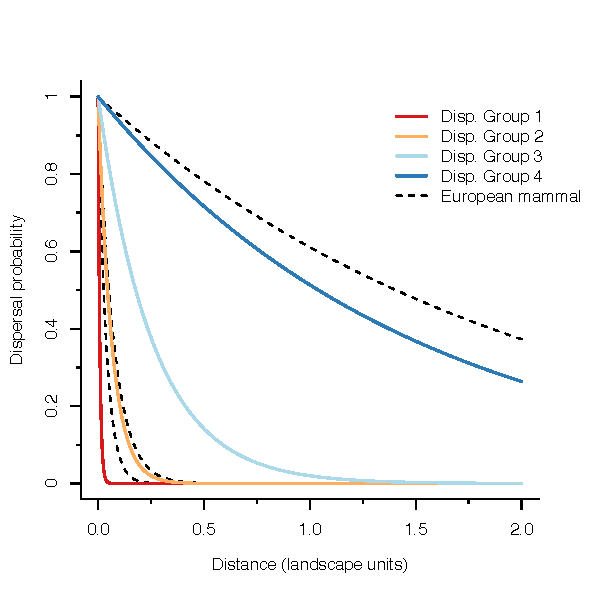
\includegraphics[width=6in]{Fig1_PlotWithLegendsMini_4mammals.pdf}
\end{center}
\caption{ }
\end{figure}

\clearpage

\begin{sidewaysfigure}[!ht]
\begin{center}
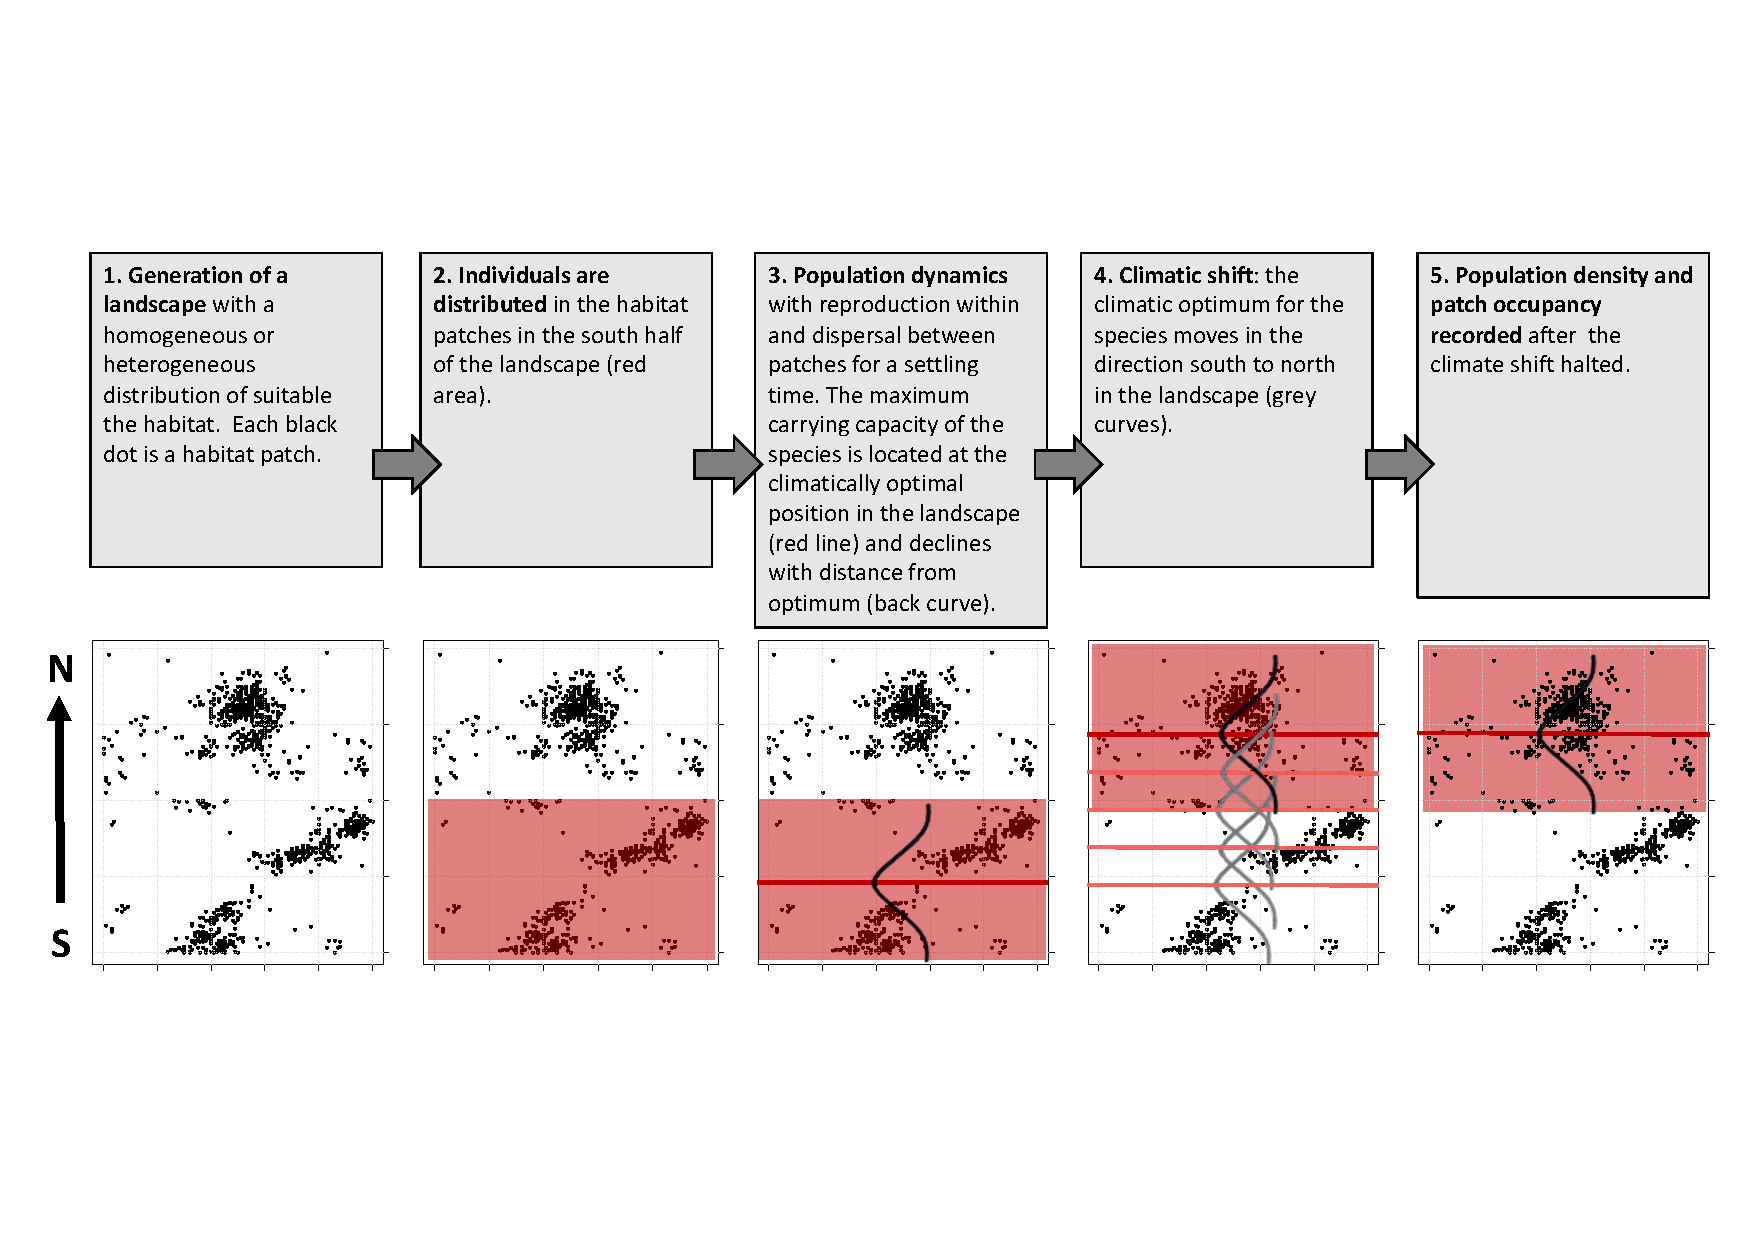
\includegraphics[width=9in]{Fig2_FlowChartRangeShift.pdf}
\end{center}
\caption{ }
\end{sidewaysfigure}

\clearpage

\begin{figure}[!ht]
\begin{center}
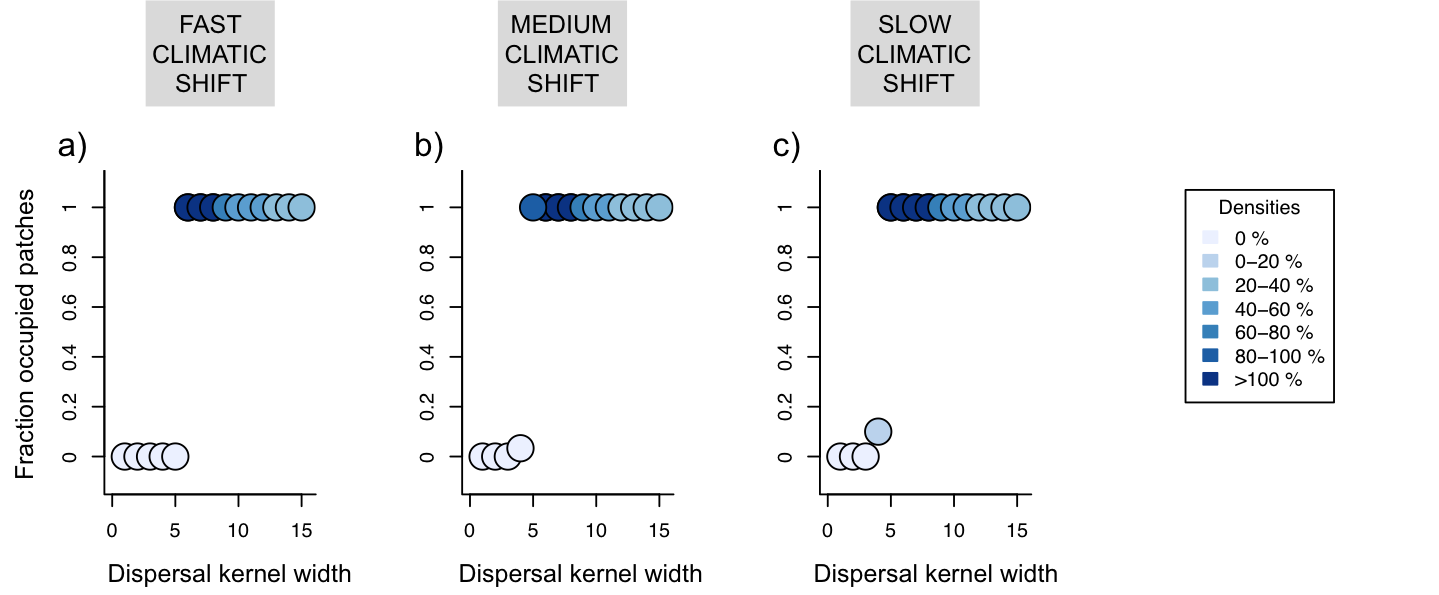
\includegraphics[width=7in]{Fig3_homo.png}
\end{center}
\caption{ }
\end{figure}

\clearpage

\begin{figure}[!ht]
\begin{center}
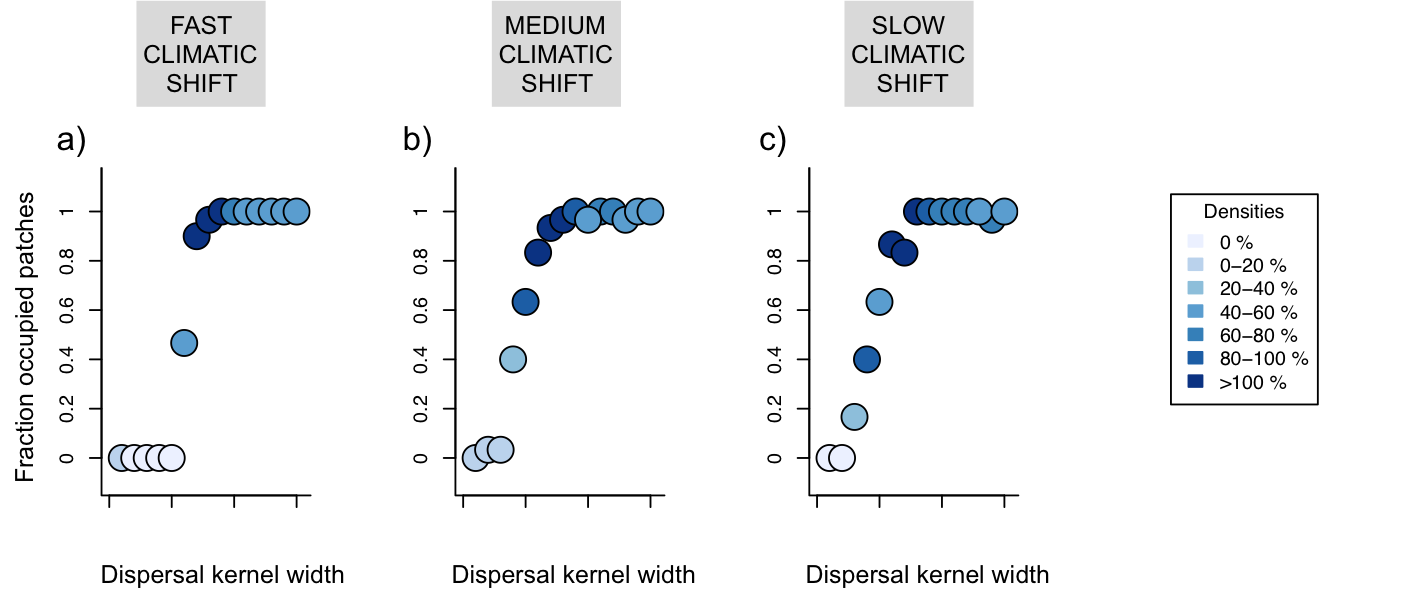
\includegraphics[width=7in]{Fig4_hetero.png}
\end{center}
\caption{ }
\end{figure}

\clearpage

\begin{figure}[!ht]
\begin{center}
\centerline{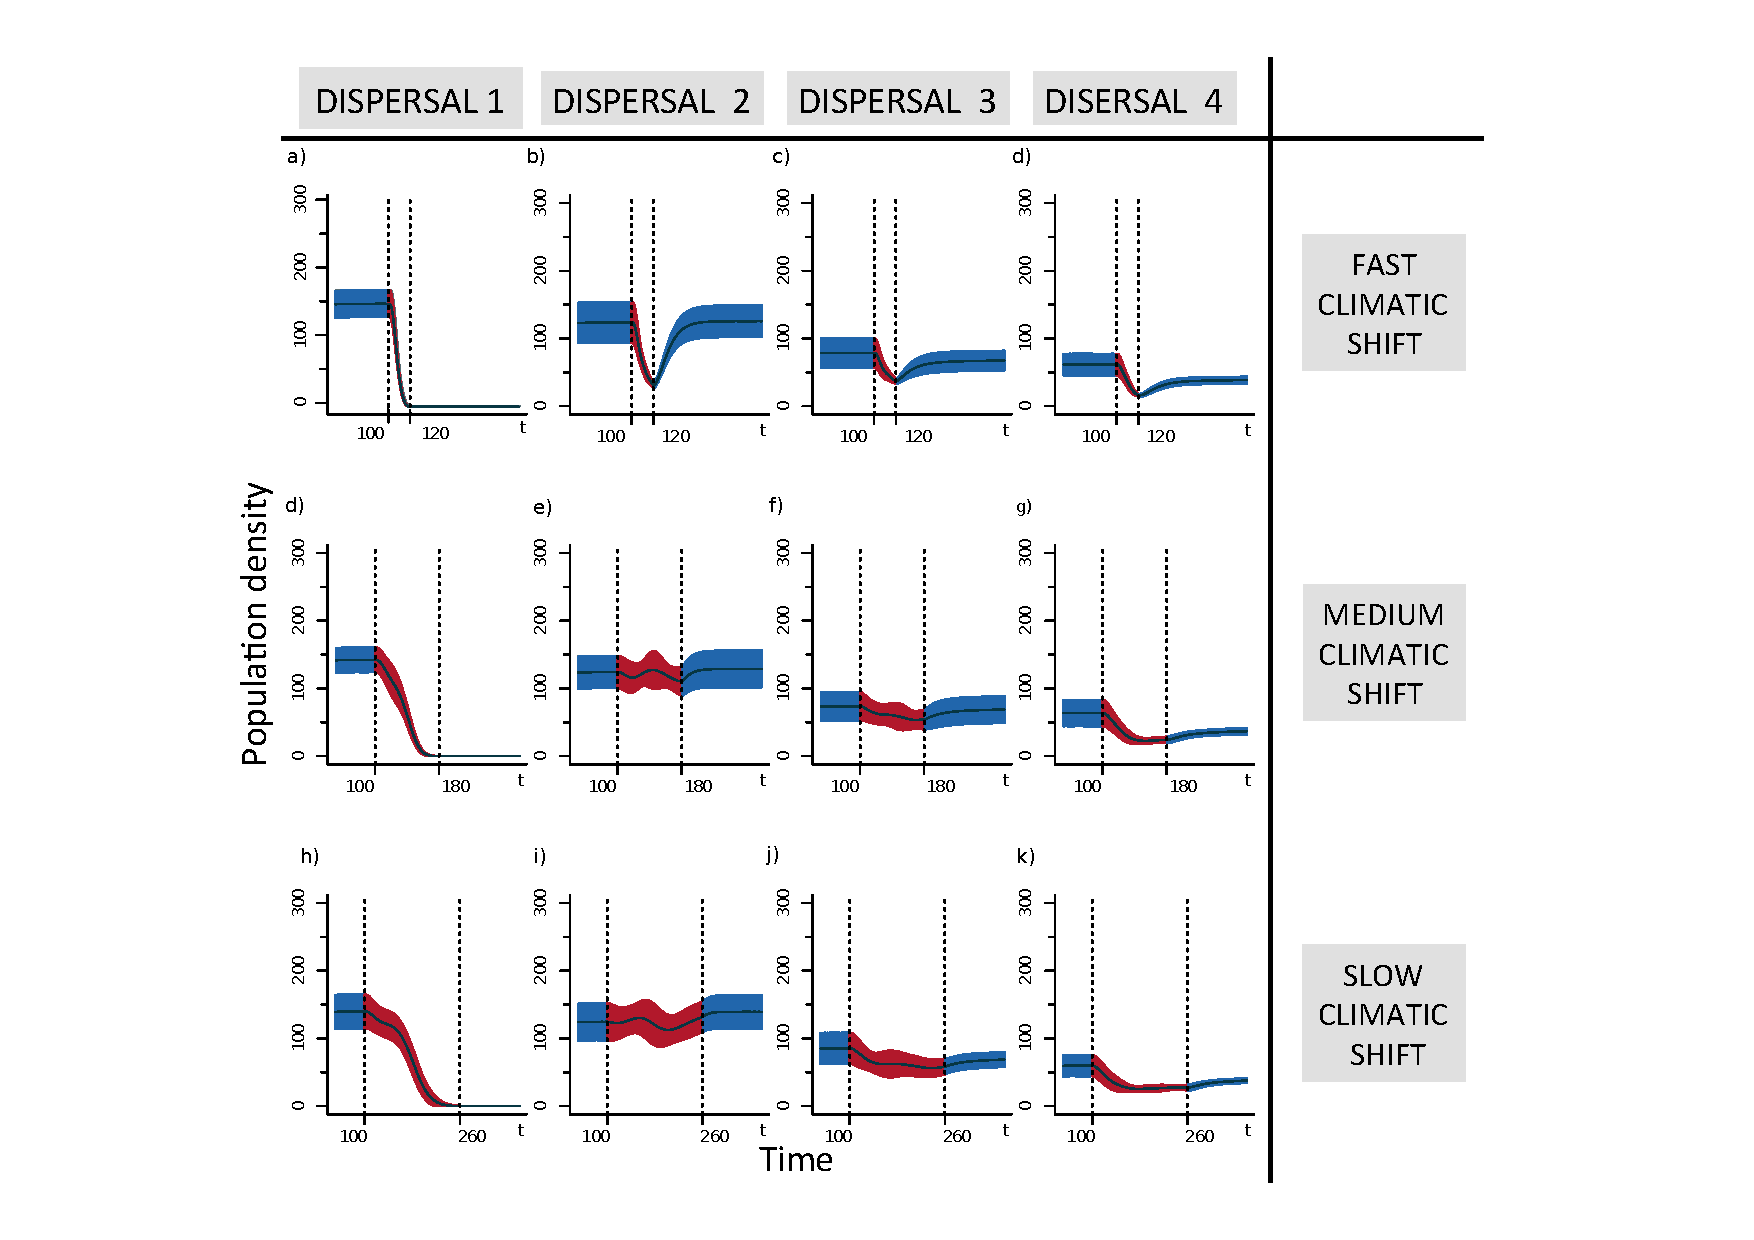
\includegraphics[width=8in]{Fig5_DensityFigHomo.pdf}}
\end{center}
\caption{ }
\end{figure}

\clearpage

\begin{figure}[!ht]
\begin{center}
\centerline{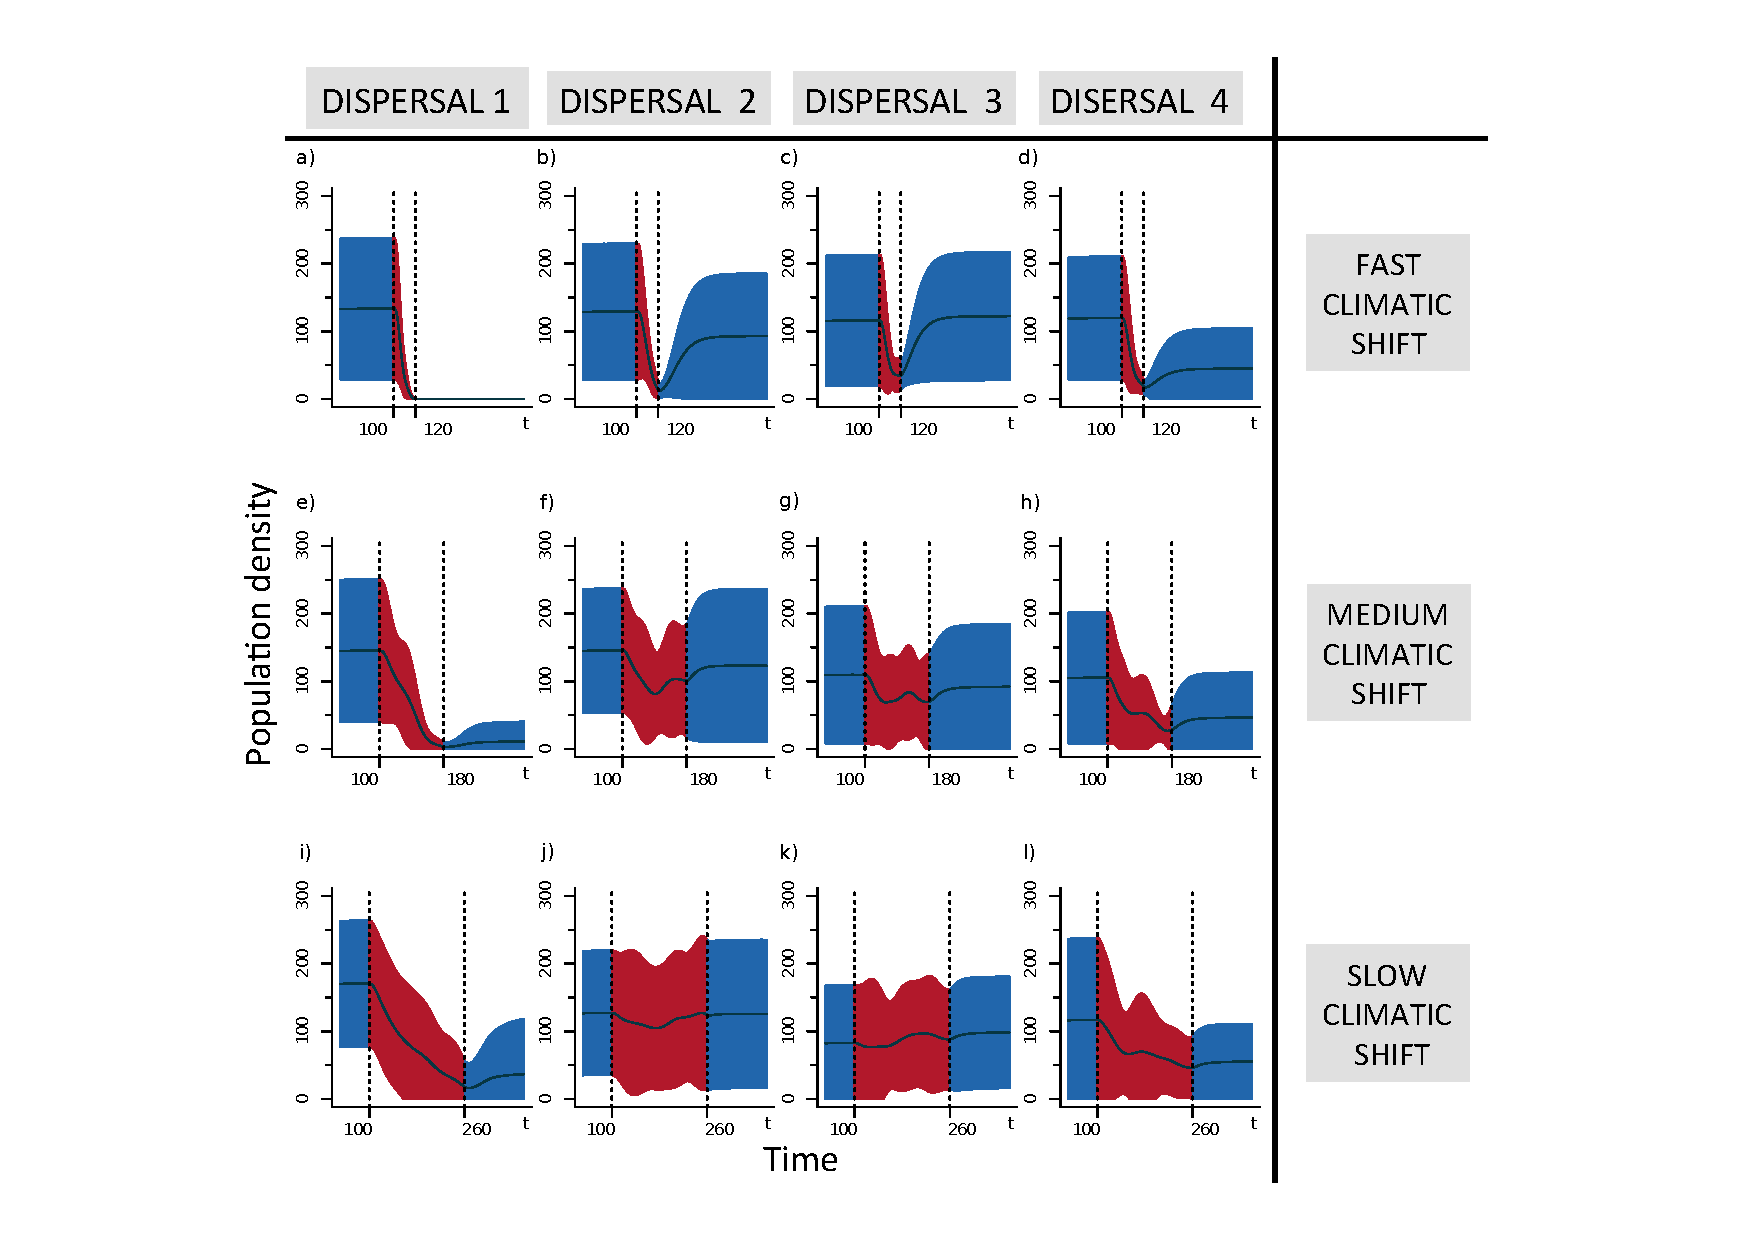
\includegraphics[width=8in]{Fig6_DensityFigHetero.pdf}}
\end{center}
\caption{ }
\end{figure}

\clearpage

\begin{table}
\begin{tabular}{lllll}
\hline
{\bf Split}						&{\bf Factor} 						&{\bf Number obs.} 					 	&{\bf Mean \# occ. patches} 	\\	
\hline
\hline
\hspace{0.00cm}	0) 			&Root 	(all data)					&720 											&399\\ 			
\hspace{0.4cm}	1) 			&DispGroup =1 					&180 										 	&32  \\
\hspace{0.8cm}  2) 			&LandscapeType=2,6A,6B 		&152 										 	&16  \\		
\hspace{1.6cm} 4) 			&LandscapeType=2 				&90 											&1 *\\		
\hspace{1.6cm} 4) 			&LandscapeType=6A,6B 		&62 										  	&37  \\		
\hspace{3.2cm} 8) 			&ShiftSpeed $<$ 120 			&39 										  	&12 *\\		
\hspace{3.2cm} 8) 			&ShiftSpeed $\geq$120 			&23 										  	&79 *\\			
\hspace{0.8cm} 2) 			&LandscapeType=6C 			&28 										 	&119  \\		
\hspace{2cm} 5) 				&ShiftSpeed $<$ 50 				&14 										  	&0.1 *\\		 
\hspace{2cm} 5) 				&ShiftSpeed $\geq$50 			&14 									 		&238 *\\		
\hspace{0.4cm} 1) 			&DispGroup=2,3,4 				&540 										 	&521  \\		
\hspace{1.2cm} 3) 			&DispGroup=2 					&180 											&465  \\		
\hspace{2.4cm} 6) 			&LandscapeType=6A,6B 		&64 										 	&410 *\\	
\hspace{2.4cm} 6) 			&LandscapeType=2,6C 			&116 									 		&494 *\\		
\hspace{1.2cm} 3) 			&DispGroup=3,4 					&360 											&549  \\		 	
\hspace{2.8cm} 7) 			&DispGroup=3 					&180 										 	&532 *\\
\hspace{2.8cm} 7)			&DispGroup=4 					&180											&566 *\\		
\hline
\end{tabular}
\caption{Regression tree explaining the number of patches occupied at the end of the simulation. Entities with * indicate terminal branches.}
\end{table}

\begin{table}
\begin{tabular}{lllll}
\hline
{\bf Split}									&{\bf Factor} 						&{\bf Number obs.} 			&{\bf Mean pop. density} 	\\ 	
\hline
\hline
\hspace{0.00cm}	0)						&Root 	(all data)				&720 							 	&45056 \\ 	
\hspace{0.4cm}   1) 						&DispGroup=1,4 				&360 							  	&19086\\ 	
 \hspace{0.8cm}    2) 						&DispGroup=1 				&180 					   			&3616 *\\		
   \hspace{0.8cm}  2) 						&DispGroup=4 				&180 							 	&34555\\	 
  \hspace{1.6cm}    4) 					&LandscapeType=2,6B,6C 	&147 							 	&26973*\\	
   \hspace{1.6cm}	4) 						&LandscapeType=6A 		&33 								&68329\\	 
     \hspace{2.4cm}   6) 					&ShiftSpeed $<$ 120 		&20 								&43689*\\	
        \hspace{2.4cm}	6) 					&ShiftSpeed $\geq$120 		&13 								&106236*\\	
\hspace{0.4cm}   1) 						&DispGroup=2,3 				&360 							  	&71026 \\	
 \hspace{1.2cm}    3) 						&ShiftSpeed $<$ 50 			&120 							  	&28767*\\	
   \hspace{1.2cm}  3) 						&ShiftSpeed $\geq$50 		&240 							  	&92156 \\	
     \hspace{2.0cm} 5) 					&DispGroup=3 				&120 							  	&67534 \\	
   \hspace{2.8cm}     7)					&LandscapeType=2,6C 		&73 								&55537*\\	
       \hspace{2.8cm} 7)					&LandscapeType=6A,6B 	&47 								&86167*\\	
     \hspace{2.0cm} 5) 					&DispGroup=2 				&120 							 	&116778 *\\	
\hline
\end{tabular}
\caption{Regression tree explaining the global population density at the end of the simulation. Entities with * indicate terminal branches. }
\end{table}


\begin{figure}[!ht]
\begin{center}
\centerline{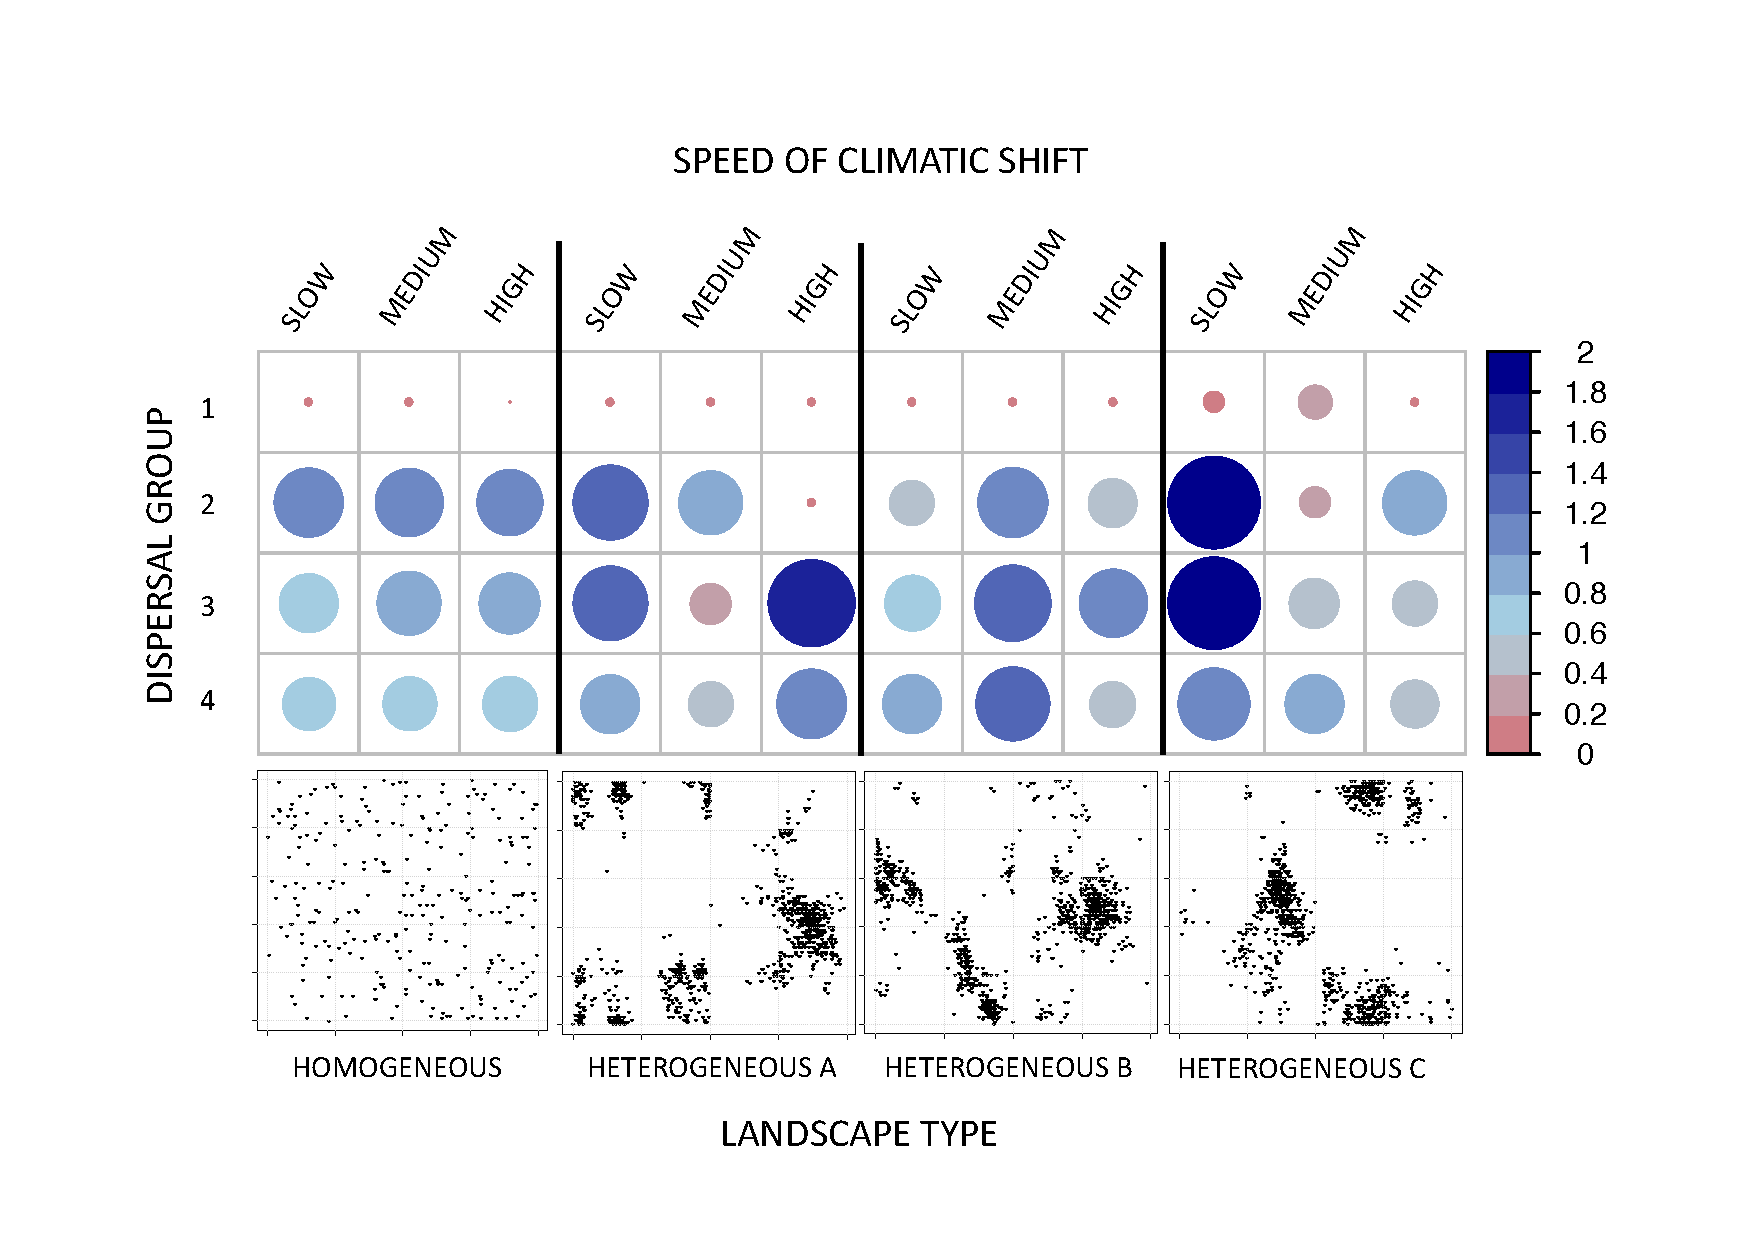
\includegraphics[width=9in]{Fig7_SummaryFigureConservationActions.pdf}}
\end{center}
\caption{}
\end{figure}

\begin{figure}
\centerline{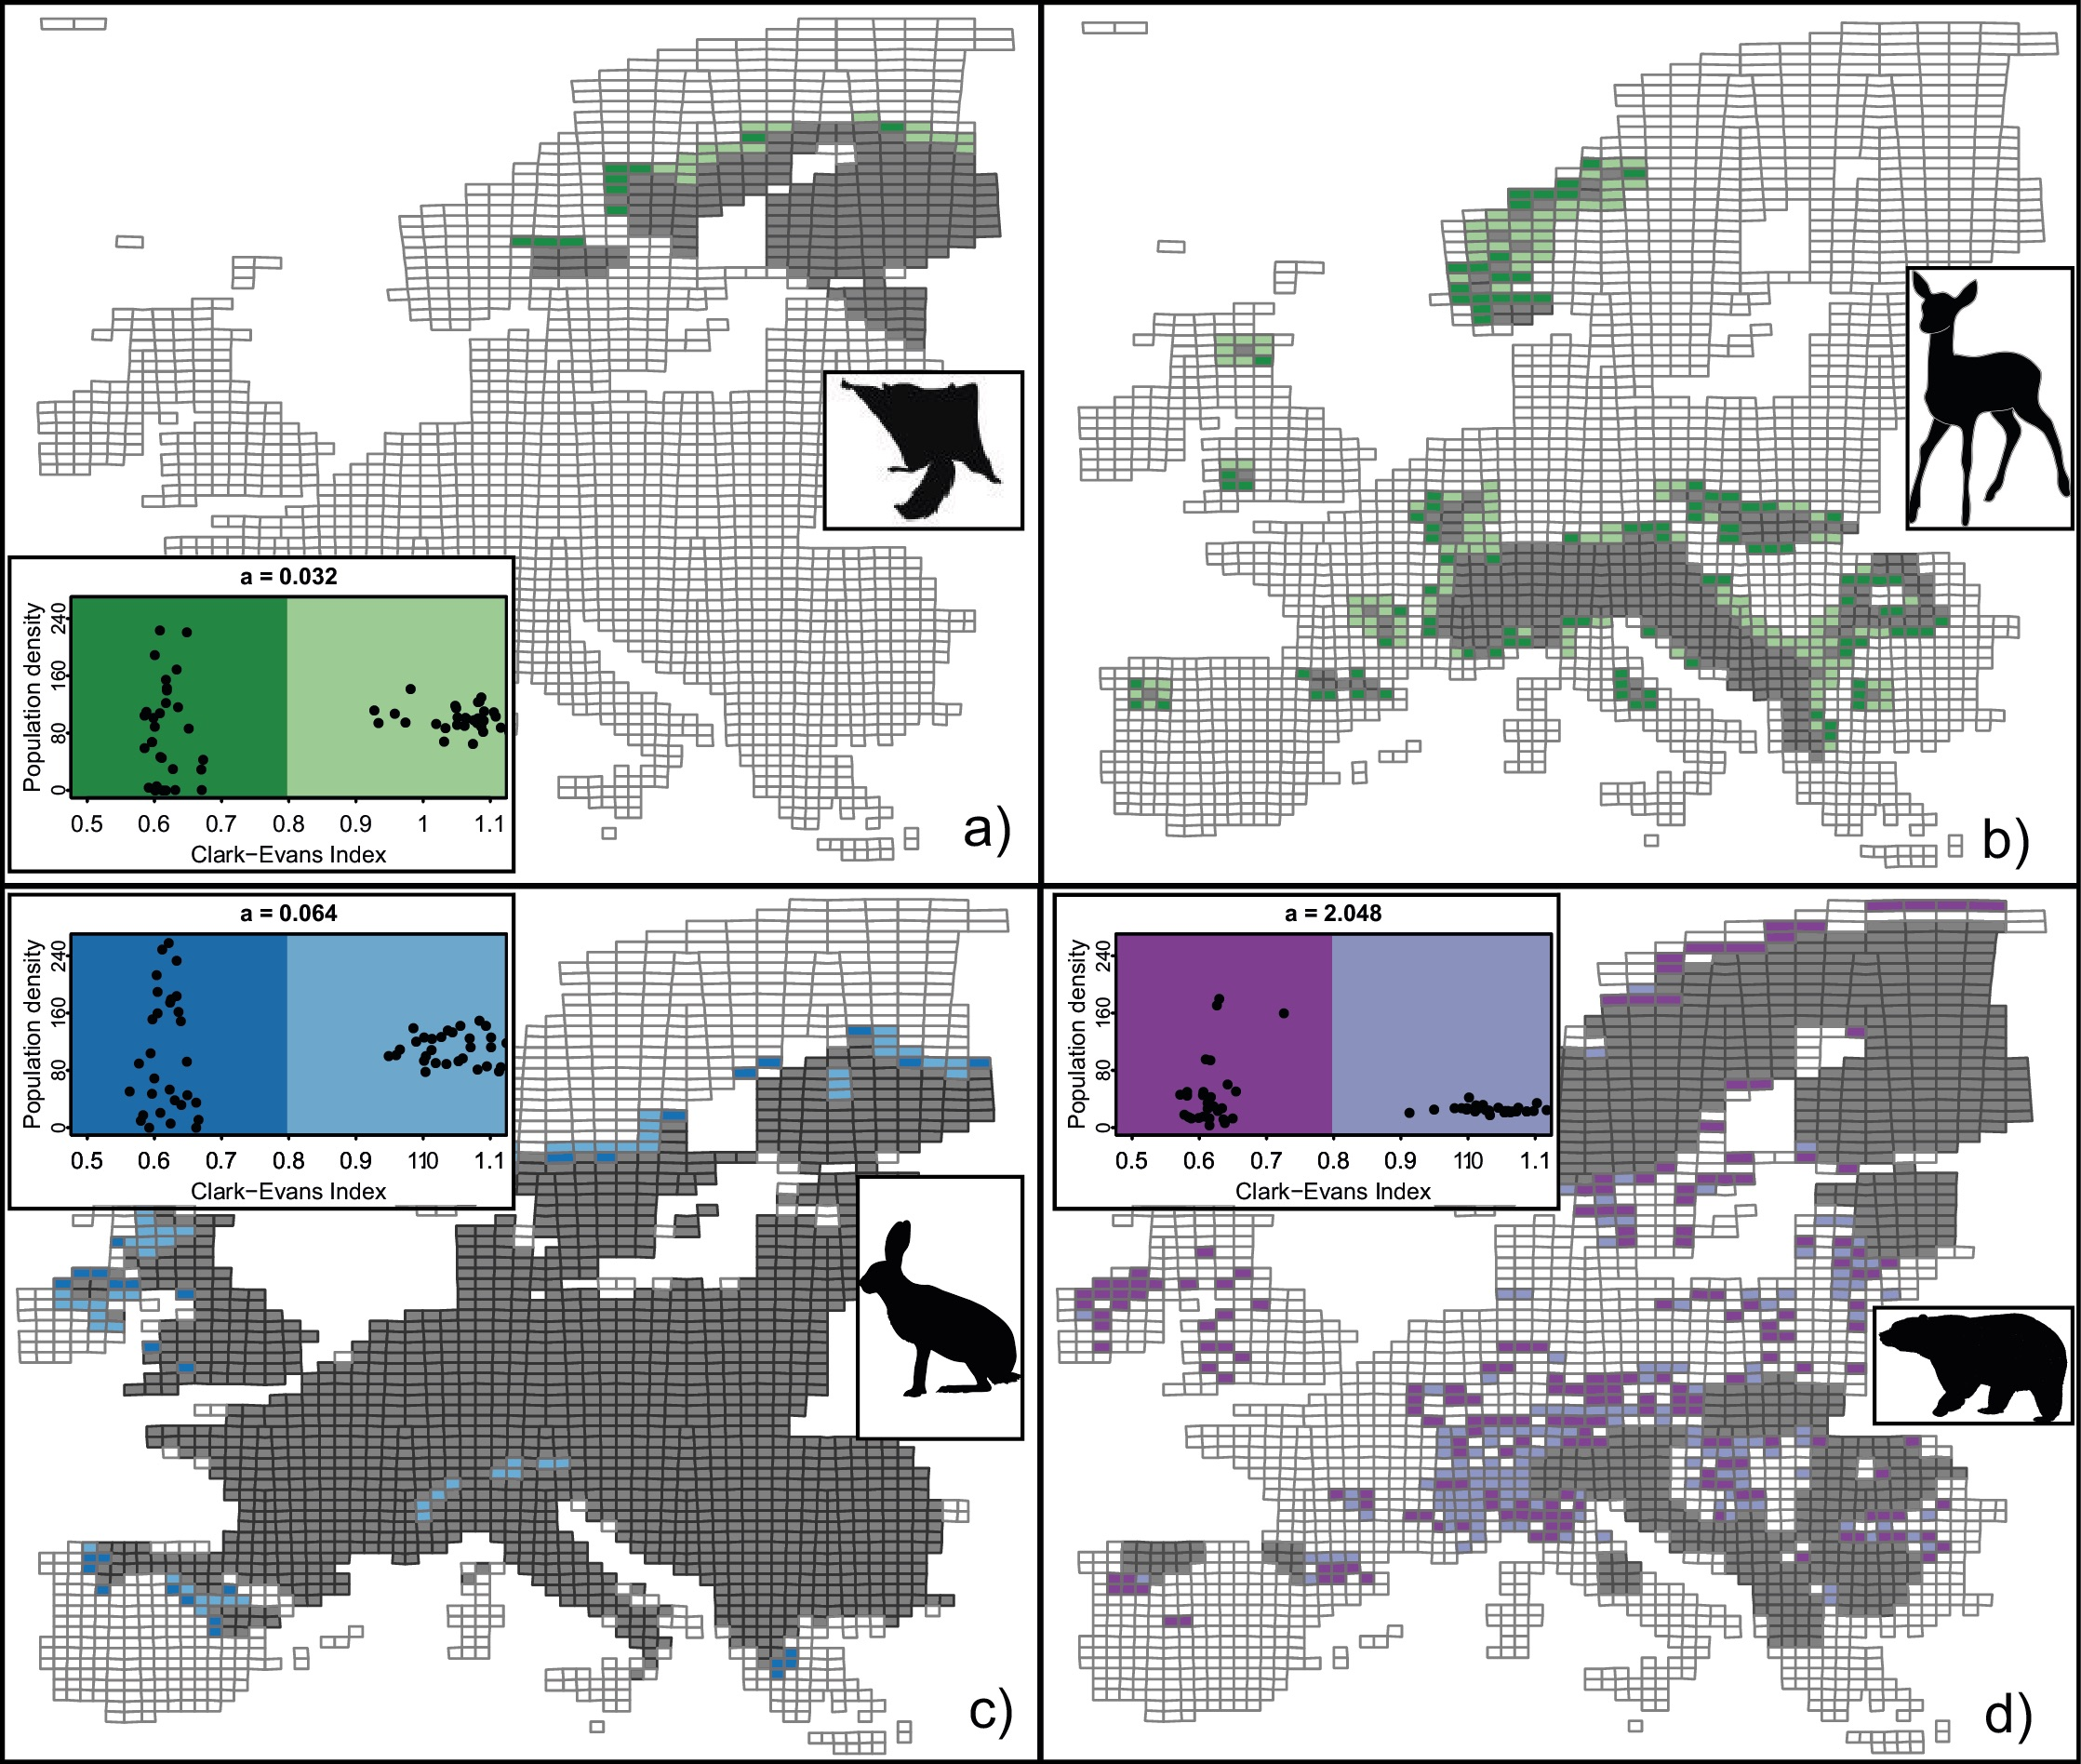
\includegraphics[width=7in]{Fig8_map_mammals.jpg}}
\caption{}
\end{figure}

\end{spacing}

\end{document}

